\RequirePackage{docswitch}
\setjournal{\flag}

\documentclass[\docopts]{\docclass}


\usepackage{lsstdesc_macros}

\usepackage{graphicx}
\graphicspath{{./}{./figures/}{.logos}}
\bibliographystyle{apj}


\newcommand{\textul}{\underline}
\newcommand{\qp}{\texttt{qp}}
\newcommand{\pz}{photo-$z$ PDF}
\newcommand{\Pz}{Photo-$z$ PDF}


\begin{document}

\title{ Approximating photo-z PDFs for large surveys }


\begin{abstract}

Upcoming and ongoing galaxy surveys will produce redshift probability 
distribution functions (PDFs) in addition to traditional photometric redshift 
(photo-$z$) point estimates.  However, the storage of \pz s may present a 
challenge with increasingly large catalogs, as we face a trade-off between the 
accuracy of subsequent science measurements and the storage cost.  This paper 
presents \qp, a Python package facilitating manipulation of approximations of 
1-dimensional PDFs, as suitable for \pz s.  We use \qp\ to investigate the 
performance of three PDF formats on two realistic datasets representative of 
upcoming surveys with different data qualities as a function of the number of 
stored parameters per \pz, using metrics of both individual \pz s and an 
estimator of the overall redshift distribution function.

\end{abstract}

\dockeys{methods: data analysis, catalogs, surveys}

\maketitlepost

\COMMENT{Consider alternative title.}




\section{Introduction}
\label{sec:intro}


Ongoing and upcoming photometric galaxy surveys such as the Large Synoptic 
Survey Telescope (LSST) will observe tens of billions of galaxies without 
spectroscopic follow-up to obtain redshifts necessary for studies of cosmology 
and galaxy evolution, instead relying on the methods of photometric redshift 
(photo-$z$) estimation.  Photo-$z$s are subject to a number of systematic 
errors, some caused by the data analysis procedures and others intrinsic to the 
data itself.  Due to these issues, the photo-$z$ community has come to favor 
estimation of redshift probability distribution functions (PDFs), or \pz s, 
that include information about the potential for such systematic errors for 
each galaxy in the survey.  \Pz s are interim posterior distributions, as they 
are estimates of the probability of a galaxy's redshift conditioned on its 
photometric data and any assumptions made by the method producing it, though 
they are commonly written simply as $p(z)$.

Given the tremendous size of the surveys in question, storage of these 
probability distributions involves making difficult decisions.  Each survey 
seeks to create a catalog of \pz s balancing accuracy against storage 
footprint.  For example, the \pz\ catalog that LSST will release is limited to 
200 floating point numbers per galaxy, with plans to store \pz s derived by 
multiple methods.  \citep{juric_data_2017}  \COMMENT{Review Tab. 5 of this 
reference.}  These matters were first addressed in 
\citet{carrasco_kind_sparse_2014} in the context of a single galaxy survey, a 
limited set of storage formats, and metrics restricted to that survey's 
intended \pz\ use case.  The number of stored parameters and the 
parametrization optimizing this choice, however, depend on the science 
requirements of the survey and the characteristics of the data.  This paper 
answers the question of \textit{how} these choices should be made in general, 
demonstrating the approach on diverse mock data and using mathematically 
motivated metrics of both the individual \pz s and a science application.  The 
publicly available \qp\ Python package is also presented here as a tool to 
enable each survey to optimize these choices.

In Sec. \ref{sec:methods}, we outline how \qp\ can be used to optimize the 
choice of storage format and catalog allocation.  In Sec. \ref{sec:data}, we 
describe the mock datasets on which we perform such an analysis.  We present 
the results of this procedure in Sec. \ref{sec:results} and make 
recommendations for the use of \qp\ by the photo-$z$ community in 
\ref{sec:conclusions}.








\section{Methods}
\label{sec:methods}



We have developed the \qp\ Python package to facilitate manipulation of \pz s.  
A \texttt{qp.PDF} object is defined by its parametrizations.  By way of 
interpolation, \qp\ can convert a representation of a \pz\ under one 
parametrization to a representation of that \pz\ under a different 
parametrization.  The currently supported parametrizations are described in 
Sec. \ref{sec:approx}.  \qp\ also includes a few built-in metrics of the 
accuracy of a representation of a \pz\ if its value under a given 
parametrization is designated as "true."  The currently implemented metrics are 
described in Sec. \ref{sec:metrics}.

\subsection{Approximation Methods}
\label{sec:approx}


First, we establish a vocabulary for the definitions of approximation methods.  
Each \textit{parametrization} of a \pz\ is defined in terms of the 
\textit{format} $\mathcal{F}$, \textit{metaparameters} comprising $\vec{C}$, 
and \textit{parameters} comprising $\vec{c}$.  Each parametrization in turn 
corresponds to a \textit{representation}
\begin{align}
  \hat{p}_{\mathcal{F}, \vec{C}}(z) &\equiv \mathcal{F}(z;\vec{C}, \vec{c})
\end{align}
of the \pz, denoted as $\hat{p}(z)$ for brevity.

\qp\ is currently capable of converting a \pz\ between the following five 
formats: step functions, samples, grid evaluations, mixture models, and 
quantiles.  These formats are described below in terms of the number $N_{f}$ of 
stored parameters $c_{i}$ per \pz, which are presumed to be floating point 
numbers unless otherwise specified.  The metaparameters are set of $N_{M}$ 
numbers $C_{m}$ necessary to convert the stored \pz\ parameters $\vec{c}$ into 
a probability distribution function over redshift.  Because the metaparameters 
for a catalog of \pz s released by a survey will only need to be stored once, 
it does not matter how large $N_{M}$ is.  For each format, we address the 
following questions:
\begin{itemize}
  \item When/where has this format appeared in the literature as a published 
catalog format, native \pz code output format, and science application input 
format?
  \item What exactly is stored under this format, per galaxy (the parameters) 
and per catalog (the metaparameters)?
  \item Beyond fidelity to the original \pz, what are the a priori strengths 
and weaknesses of this format, especially with respect to 
compression/reconstruction properties?
\end{itemize}

\begin{figure}
  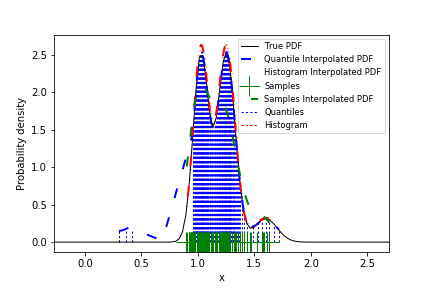
\includegraphics[width=0.9\columnwidth]{figures/qp_placeholder.png}
  \caption{Placeholder! [all available $\hat{p}(z)$ for one \texttt{qp.PDF} 
object and given $N_{f}$; show multiple \texttt{qp.PDF} objects? multiple 
$N_{f}$? realistically complex or simple Gaussian?]
  \label{fig:qp}}
\end{figure}

\subsubsection{Regular Binning}
\label{sec:bins}

By far the most popular format for \pz s is that of a piecewise constant step 
function, also called a histogram binning.  It is the only format that has been 
used for public release of \pz\ catalogs \citep{tanaka_photometric_2017, 
sheldon_photometric_2012}; it is unclear whether this is a consequence or a 
cause of the fact that it is the most common format for using \pz s in 
cosmological inference, as tomographic binning is a universal step between the 
\pz\ catalog and calculation of any two-point correlation function.

The metaparameters of the binned parametrization are the ordered list of 
$N_{M}=N_{f}+1$ redshifts $(z_{1}, z_{2}, \dots, z_{N_{M}-1}, z_{N_{M}})$ with 
$z_{1} < z_{2} < \dots < z_{N_{M}-1} < z_{N_{M}}$ and 
$z_{m+1}=z_{m}+\Delta_{m}$ serving as endpoints shared by all galaxies in the 
catalog, each adjacent pair of which is associated with a parameter 
$c_{i}=\int_{z_{i}}^{z_{i+1}}p(z)dz$.  If the binning is "regular," then 
$z_{i+1}=z_{i}+\Delta$ for some constant scalar $\Delta$.  As this is the only 
type of binning that has been used in the literature, it is the only one we 
consider.  The standard assumption that $p(z)=0$ when $z<z_{1}$ or 
$z>z_{N_{M}}$ implies that the $c_{i}$ are normalized according to $\sum_{i} 
c_{i}\cdot\Delta = 1$.  Note that this is not equivalent to the erroneous 
normalization condition $\sum_{i} c_{i} = 1$ that commonly appears in the 
literature.  The \pz\ under this representation is thus
\begin{align}
  \label{eq:bin_interpolated}
  \hat{p}(z) &= \left\{\begin{tabular}{cc}$z_{i}<z<z_{i+1}$&$c_{i}$\\
$z < z_{i}$\ or\ $z > z_{i+1}$&$0$\end{tabular}\right\}.
\end{align}

All known native \pz\ formats are easy to convert to the histogram 
representation.  However, the corrolary to this statement is that it is an 
inherently lossy format.  A \pz\ with features smaller than the bin width may 
not accurately represent the underlying probability distribution, as 
significant structure may be stored as a single bin value.  This problem may be 
particularly troubling as the quality of the approximation may not be unbiased 
among catalog entries; rather, it is likely to correlate with the properties of 
the \pz\ in question and thus the true redshift of the galaxy.

The binned parametrization may also be considered wasteful in terms of data 
storage.  A \pz\ with a compact probability distribution, with much of the 
probability contained within a region far narrower than the redshift range 
$z_{N_{M}} - z_{1}$, may have many of its catalog entries $c_{i}$ being 
identically zero.  The storage footprint of this data is wasted in that it is 
redundant, with each $c_{i}$ requiring the same space even though 
$c_{i}=c_{i'}$ for many pairs $(i, i')$.

Finally, the binned parametrization requires the researcher to choose the 
minimum and maximum possible redshifts of the galaxy sample.  These are 
physical quantities that are unknown, so it would be preferable to not have to 
choose them at the stage of producing the \pz\ catalog.

\subsubsection{Samples}
\label{sec:samples}

Samples $(z_{1}, z_{2}, \dots, z_{N_{f}-1}, z_{N_{f}})$ are another common 
storage format for \pz s.  Samples are the native output format of many machine 
learning algorithms dependent on random choices, such as random forests.  Such 
approaches typically produce large numbers of samples, far more than can 
realistically be stored by any survey, so a subsample is commonly stored.  
\COMMENT{Cite upcoming DES paper.}

A small number of samples from a broad \pz may not be representative of the 
overall shape, boosting the variance across the catalog, but it can be 
appropriate for \pz s with narrow features.  As in the case of the histogram 
parametrization, the quality of the approximation may be correlated to 
properties of the \pz that themselves correlate with redshift.  Unlike the 
simple reconstruction scheme for the histogram format (Eq. 
\ref{eq:bin_interpolated}), there is no straightforward interpolation for 
samples.  When we need one for the purposes of calculating metrics, we use a 
kernel density estimate, which may introduce additional loss of information.  
\COMMENT{Expand on details here.}

Though it is possible to construct a catalog where each galaxy has a different 
number $N_{f}$ of stored samples, optimizing the choice of $N_{f}$ given the 
shape of the \pz\ in its native format is nontrivial.  As this has not been 
done in the literature, we leave its investigation to future work.

\subsubsection{Evaluation on a Regular Grid}
\label{sec:grid}

\COMMENT{Should I discuss this since it isn't one of the three I test?}

Another storage option is evaluations of a continuous functional form of a \pz\ 
at $N_{f}$ redshifts $(z_{1}, z_{2}, \dots, z_{N_{f}-1}, z_{N_{f}})$.  Thus 
far, only a regular grid of redshifts (i.e. $z_{i+1}=z_{i}+\Delta$ for a 
constant $\Delta$) shared among the entire catalog have been used in the 
literature, so we do not consider irregular grids or grids that are not 
homogeneous over the catalog.   In some cases, this is the native output format 
of a \pz\ code.  For example. template-fitting codes may populate the template 
library with colors of each SED evaluated on a regular grid of redshifts for 
computational efficiency.

The gridded parametrization is in some ways similar to the histogram format of 
\ref{sec:bins}, suffering from the same risks of losing small-scale features 
(and the corresponding risk of systematics in the quality of the 
approximation), wasting a substantial fraction of the $N_{f}$ allocated 
parameters, and choosing the grid endpoints.  Like the piecewise constant 
parametrization, the grid evaluations may need to be normalized before they can 
be used as a mathematically valid \pz.  Relative to the histogram format, it 
can be challenging to convert to this format from the native format of a \pz\ 
code, as it requires a continuous function for the \pz.  On the other hand, it 
is easy to reconstruct a continuous $\hat{p}(z)$ by interpolating the gridded 
values.  In this paper we use linear interpolation.  \COMMENT{Expand on this.}

\subsubsection{Mixture Model}
\label{sec:mm}

\COMMENT{Should I discuss this since it isn't one of the three I test?}

There is some history of using a mixture model parametrization for \pz s.  
\COMMENT{Seek citation.}  In this work, we consider only the common Gaussian 
mixture model, though the \qp\ framework can accommodate mixtures of all 
probability distribution functions that have been implemented as 
\texttt{scipy.stats.rv\_continous} objects.

A Gaussian mixture model may be a natural choice for the native output of a 
template-fitting code or one based on a distance metric in the space of 
photometry because the \pz s could be weighted sums of Gaussians by 
construction; for many other methods, however, there is no such guarantee.  The 
mixture model is only an accurate approximation of the \pz s are actually 
comprised of components of the included parametrizations.  As with the gridded 
approximation, the challenge of compressing an original $p_{0}(z)$ into this 
format is balanced by the ease of reconstructing an estimated $\hat{p}(z)$ from 
its stored parameters, as no interpolation is even necessary.

Besides the mixture of Gaussians, other functions have been investigated before 
in the sparse basis representation of \citet{carrasco_kind_sparse_2014}, which 
uses a mixture model of members of a library of $N_{M}\sim10^{4}$ functions.  
Though it has promising compression properties, we do not consider it in this 
work for several reasons.  Decomposition with \texttt{SparsePZ} does not 
enforce that the stored parametrization be a probability distribution in the 
mathematical sense of always being positive semidefinite and integrating to 
unity, which is a necessary condition for \qp.  While normalizing a positive 
semidefinite function to integrate to unity is always possible, one can devise 
multiple schemes for enforcing nonnegativity that result in different 
reconstructions $\hat{p}(z)$.   We anticipate including the sparse basis 
representation in \qp\ in future work when we can justify a choice of how to 
handle negative values and avoid compounding format conversions.


\subsubsection{Regular Quantiles}
\label{sec:quantiles}

One parametrization that has not previously been implemented is that of 
quantiles, which are defined in terms of the cumulative distribution function 
(CDF)
\begin{align}
  \label{eq:cdf}
  CDF(z) &= \int_{-\infty}^{z}\ p(z)\ dz.
\end{align}
Under the quantile parametrization, an ensemble of \pz s shares a set of 
$N_{f}$ values $0<q_{1}<q_{2}<\dots<q_{N-1}<q_{N_{f}}<1$.  Each galaxy's 
catalog entry is the $N_{f}$ values $z_{i}$ satisfying $CDF(z_{i})=q_{i}$.  In 
our tests, the quantiles are regular, such that $q_{i}\equiv i\bar{q}$, where 
$\bar{q}\equiv(N_{f}+1)^{-1}$, but \qp\ does not require that this be so.

The quantile parametrization is the inspiration for this work and namesake of 
\qp.  Though it has not appeared in the \pz\ literature prior to this point, it 
is a natural choice for the compression of probability distributions because it 
keeps more information in areas of higher probability density, so there is 
inherently less waste in the information that is stored for each catalog entry 
and minimal risk of bias in the quality of the approximation across \pz\ 
shapes.  Storing quantiles is equivalent to storing piecewise constant data (or 
function evaluations) on an irregular binning (or irregular grid) optimized to 
have narrower bins (denser evaluations) in areas of high probability and wider 
bins (more diffuse evaluations) in areas of low probability, effectively 
performing the optimization in bin size (grid resolution) while still 
permitting an entire catalog to share a single set of metaparameters.  Unlike 
samples, it is guaranteed to be an equally good approximation regardless of the 
shape of the \pz.

The strengths and weaknesses of quantiles have not yet been explored, as no 
survey has previously stored quantile \pz s, no existing \pz\ code produces 
quantiles as output, and no science case pipeline has yet been developed to 
accept input \pz s as quantiles.  We can, however, comment on matters of 
compression and extraction.  Some native \pz\ output formats, like samples, are 
easy to convert to regular quantiles, while others, like piecewise constant 
functions, are not, requiring a numerical optimization for each parameter $i$.  
Reconstruction of an approximate \pz\ $\hat{p}(z)$ requires a choice of 
interpolation scheme and choices about the probability density for $z<z_{1}$ 
and $z>z_{N_{f}}$.  Nonetheless, the quantile parametrization is a new option 
that merits careful consideration.

\subsection{Comparison Metrics}
\label{sec:metrics}

We use two metrics to quantify how well an approximation of a \pz\ extracted 
from a stored format represents the original \pz, characterized by many more 
parameters than are available for storage, before it was compressed.  In 
contrast to popular \pz\ metrics in the literature, this study aims to probe 
how well an approximation of $p(z)$ represents an original $p(z)$, so there is 
no notion of the accuracy of either the approximation nor the original $p(z)$ 
relative to a galaxy's true redshift.  (For a demonstration of how one might 
approach the different problem of evaluating the accuracy of a \pz\ relative to 
a true redshift, see Schmidt, et al. (in prep.).)

For most galaxy surveys producing \pz\ catalogs, it is important to reconstruct 
individual \pz s.  For example, they may be used as the basis for targeting 
spectroscopic follow up for a variety of science applications.  However, \pz s 
have thus far been used almost exclusively to estimate the redshift 
distribution function $n(z)$ necessary for calculating the correlation 
functions used by many cosmological probes.  In addition to comparing the 
properties of the distributions of individual \pz\ metrics, we also calculate 
the metrics on an estimator $\hat{n}(z)$ of the redshift distribution function 
$n(z)$, which is itself a 1-dimensional PDF.  The most common way to estimate 
the redshift distribution function is to sum the \pz s according to
\begin{align}
  \label{eq:nz}
  \hat{n}(z) &\equiv \frac{1}{N_{g}}\ \sum_{j=1}^{N_{g}}\ \hat{p}_{j}(z),
\end{align}
where the estimator is normalized so that it, too, is a probability 
distribution.  Though we do not recommend this approach to estimating the 
redshift distribution (see Malz and Hogg, et al. (in prep.) for a 
mathematically consistent alternative), we calculate the metrics below on this 
"stacked estimator" of the redshift distribution function under the assumption 
that inaccuracy and imprecision of an alternative estimator $\hat{n}'(z)$ 
behaves similarly to that of the stacked estimator $\hat{n}(z)$ under each 
format and number of parameters.

To calculate the metrics for a stored parameters $\vec{c}$ of a \pz\ 
approximation, we perform an interpolation to evaluations of the approximated 
\pz\ $\hat{p}(z)$ on a fine grid $(z_{1}, z_{2}, \dots, z_{N_{ff}-1}, 
z_{N_{ff}})$ and compare the approximation to the true \pz\ $p_{0}(z)$ 
evaluated on that grid, which is a mixture model by construction.  The 
distributions of metric values for each parametrization are compared in Sec. 
\ref{sec:individual}.  The metrics calculated on the stacked estimator of the 
redshift distribution function of a survey may be found in Sec. 
\ref{sec:stacked}.

\subsubsection{RMSE}
\label{sec:rms}

\COMMENT{Remove this metric from the final version after some restructuring.}

The root mean square error (RMSE) is a familiar measure of the difference 
between two functions $p(z)$ and $\hat{p}(z)$,
\begin{align}
  \label{eq:rmse}
  RMSE &= \frac{1}{N_{ff}}\ \sum_{i=1}^{N_{ff}} (p(z_{i}) - \hat{p}(z_{i}))^{2}.
\end{align}
The RMSE is symmetric in that it is simply about the difference between the 
functions, not some distance from one to the other.  The RMSE is also not 
specific to probability distributions.  The RMSE is always positive, and a 
smaller value indicates better agreement between the approximation and the 
truth.

\subsubsection{KLD}
\label{sec:kld}

The Kullback-Leibler divergence (KLD)
\begin{align}
  \label{eq:kld}
  D(p_{0}(z) || \hat{p}(z)) &= \int_{-\infty}^{\infty}\ p_{0}(z)\ 
\log\left[\frac{p_{0}(z)}{\hat{p}(z)}\right]\ dz\\
  &\approx \sum_{z_{1}}^{z_{N_{ff}}}\ p_{0}(z)\ 
\log\left[\frac{p_{0}(z)}{\hat{p}(z)}\right]\ \cdot\ \Delta
\end{align}
quantifies the loss of information of an approximation of a probability 
distribution from the true probability distribution.  The KLD is the most 
natural metric for comparing an approximation of a PDF to a true PDF and so is 
ideal for this application.

Note that the KLD is not symmetric and requires not only that both functions be 
true probability distributions but also that there must be some notion of a 
true reference distribution.  The former condition is not always satisfied for 
the binned, gridded, and mixture model formats produced by \pz\ codes; while 
\qp\ checks these conditions before attempting to calculate any metric, 
enforcing them on an approximate \pz is not always well-defined.

Though the KLD is hardly unheard of in astronomy, it is far from established.  
It is obvious that the KLD is always positive, and a smaller value indicates 
better agreement between the approximation and the truth.  The following 
discussion, however, is intended to deepen the reader's intuition for this 
metric, as it is central to the proposed procedure for choosing the best 
storage parameters for \pz\ catalogs.

\COMMENT{Add the discussion of "precision" and "tension" for single Gaussians 
as outlined in the KLD Jupyter notebook in the documentation.}


\section{Photo-z Test Data}
\label{sec:data}

With the expectation that \qp\  may suggest a different optimal result for 
different datasets, we apply it to two mock datasets with different data 
quality properties.  For example, one can expect storing a small number of 
samples to be sufficient for unimodal \pz s with low variance but disastrous 
for broader \pz s, or storing the components of a Gaussian mixture model to 
only be appropriate when the \pz s in the catalog are in fact weighted sums of 
Gaussians as opposed to other functional forms.  For this reason, we 
demonstrate the procedure for making a good choice of format and number of 
parameters on a pair of mock datasets intended to be realistic projections of 
anticipated data from upcoming surveys with different data quality.

Both datasets were fit using the publicly available Bayesian Photometric 
Redshift (BPZ) code \citep{benitez_bayesian_2000}, which employs spectral 
energy distribution (SED) fitting to a template set.  However, the choice of 
\pz\ estimation method is not relevant to this study; so long as the mock \pz s 
are realistically complex, meaning they take shapes we expect to see in 
accurate \pz s from real datasets with similar photometric properties, it does 
not matter how accurately they describe the probability distribution of galaxy 
redshifts given their photometric data.  We only seek to optimize the fidelity 
of the stored \pz\ relative to the \pz\ output by a representative \pz\ fitting 
code.  (Other work has been done to compare the accuracy of \pz s produced by 
different methods; see Schmidt, et al. (in prep.), 
\citet{tanaka_photometric_2017}.)  As BPZ is a widely used and well established 
method, we assume that the \pz s produced by it are of realistic complexity.

The mock datasets considered here begin in a gridded parametrization.  Because 
we believe that each galaxy has a true redshift interim posterior probability 
distribution that is a continuous function, to which the output of a \pz\ code 
is itself a high-resolution approximation, we fit each \pz\ in the catalog of 
densely evaluated gridded evaluations with a Gaussian mixture model, which we 
designate as $p_{0}(z)$.

\begin{figure}
  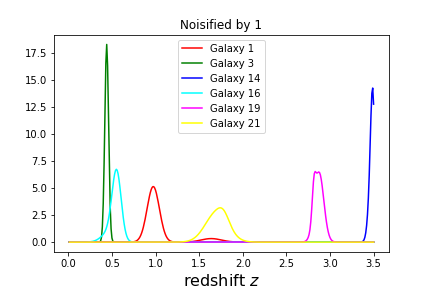
\includegraphics[width=0.9\columnwidth]{figures/pz_placeholder.png}\\
  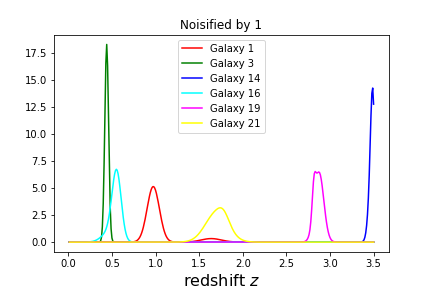
\includegraphics[width=0.9\columnwidth]{figures/pz_placeholder.png}
  \caption{Placeholder! [plot with a few examples of what the \pz s look like, 
one panel per dataset (vertical); random sample? cherrypick weirdest? how many?]
  \label{fig:pzs}}
\end{figure}

\subsection{LSST-like mock data}
\label{sec:LSST}

In order to simulate the expected LSST galaxy sample, we use the 
Buzzard-highres-v1.0 mock galaxy catalog \COMMENT{How do we cite this?}, which 
adds galaxies with SEDs drawn from an empirical library of \sim500,000 SEDs 
from the Sloan Digital Sky Survey  (SDSS) \COMMENT{Look up the spec-z sample 
reference.}  \COMMENT{Invite Joe DeRose (and Buzzard team) to review and 
contribute to this section.}  Given an SED, redshift, and absolute r-band 
magnitude for each galaxy, we compute the expected apparent magnitudes and 
magnitude errors in the six broadband LSST filters (ugrizy), assuming full 
10-year depth of the survey using the simple model of 
\citet{ivezic_lsst:_2008}.  The catalog contains 111,171 galaxies to a depth of 
$i<26.9$, 1.5 magnitudes deeper than the expected "LSST Gold sample'' of 
galaxies that will have S/N$\gtrsim$30 in multiple bands.

In implementing BPZ, we create a custom Bayesian prior using a subset of the 
Buzzard-highres-v1.0 catalog, and create a spanning template set via a simple 
k-means clustering algorithm, selection 100 of the SDSS SEDs used in creating 
the Buzzard catalog.  BPZ outputs the marginalized redshift posterior on a 
regular grid of test redshifts, in this case we have 211 points spanning 
$0.005\leqz\leq2.105$.

Even with six filters spanning the optical, there are known degeneracies 
(e.~g.~the Lyman/Balmer break degeneracy) that lead us to expect the presence 
of multi-modal \pz's; some examples are shown in the top panel of 
Fig.~\ref{fig:pzs}.  We produce "true" underlying \pz s by fitting a 
five-component Gaussian mixture model to each \pz output by BPZ.


\subsection{Euclid-like mock data}
\label{sec:Euclid}

\COMMENT{Ask for larger subset comparable to Sec. \ref{sec:LSST}.}

We start with a 30,000 object subset of the same simulated galaxy catalog used 
for LSST photometric redshift experiments by Graham, et al. (in prep.), which 
is based on the Millennium simulation \citep{springel_simulations_2005}, in 
particular the LC DEEP Gonzalez2014a \COMMENT{Fix this reference.} catalog 
based on the galaxy formation models of \cite{gonzalez-perez_how_2014}, and was 
created using the lightcone construction techniques described by 
\cite{merson_lightcone_2013}.  We limit the sample to galaxies with a catalog 
$i$-band magnitude of $i<25$ and true redshifts $z<3.5$. As in Graham, et al. 
(in prep.) we simulate observed apparent magnitudes from the true catalog 
magnitudes by adding a normal random scatter with a standard deviation equal to 
the predicted magnitude error for each galaxy (from Section 3.2.1. of 
\citealt{ivezic_lsst:_2008}, using the software of 
\citealt{connolly_end--end_2014}, assuming a mean airmass of 1.2 and a 10-year 
accumulation of 56, 80, 184, 184, 160, and 160 visits in filters $ugrizy$, 
respectively).  We also ignore any magnitudes fainter than the predicted 
10-year limiting magnitudes in each filter, $u<26.1$, $g<27.4$, $r<27.5$, 
$z<26.1$, and $y<24.9$, as a realistic simulation of non-detections.

The \pz s for this simulated catalog use the CFHTLS set of spectra 
\citep{ilbert_accurate_2006} and all of the default parameter settings for BPZ, 
except that we impose a maximum photometric redshift of 3.5 and allow BPZ to 
use the $i$-band as a magnitude prior during the photo-$z$ fit. The \pz s from 
BPZ are in the form of $N_{ff} = 351$ floating point numbers represing the 
probability on a regular grid of redshifts $0.01 < z_{\rm phot} < 3.51$.  We 
produce "true" underlying \pz s by fitting a three-component Gaussian mixture 
model to each \pz output by BPZ.



\section{Results \& Discussion}
\label{sec:results}


In this study, we perform tests comparing the parametrizations of Sec. 
\ref{sec:approx} as a function of the number of parameters per galaxy.  The 
tests are conducted using the functionality of the \texttt{qp.Ensemble} class 
that is a wrapper for collections of \texttt{qp.PDF} objects.

\subsection{Individual \pz s}
\label{sec:individual}

Parametrizations are compared on the basis of the distributions of the metrics 
of Sec. \ref{sec:metrics} calculated over all galaxies in the ensemble.  An 
example of the distribution of the KLD for $N_{f}=10$ is shown in Fig. 
\ref{fig:individual}.

\begin{figure}
  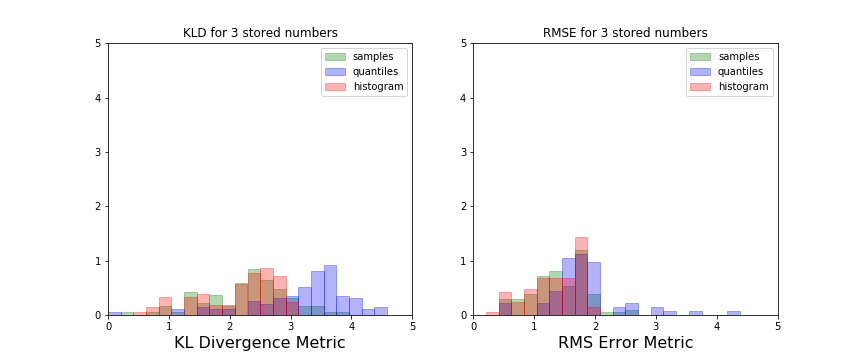
\includegraphics[width=0.9\columnwidth]{figures/individual_placeholder.png}
  \caption{Placeholder! [histogram of log-KLD for one number of parameters 
$N_{f}$, one color per format, one panel per dataset (vertical), panel title of 
(dataset, $N_{f}$)]
  \label{fig:individual}}
\end{figure}

As viewing the histograms of metric values is not especially informative, we 
compare the moments of the distributions of metric values for the individual 
\pz s under each parametrization.

\begin{figure}
  \caption{\COMMENT{Make a placeholder!} [$N_{f}$ (horizontal) vs. first few 
moment values each with separate vertical scale(?), one marker shape per moment 
(might be too confusing with many moments, will need to see which are most 
informative), one color per format, one panel per dataset (vertical), panel 
title of dataset]
  \label{fig:moments}}
\end{figure}

\COMMENT{How does moment behavior differ between datsets?}

\subsection{Stacked $\hat{n}(z)$ estimator}
\label{sec:stacked}

Parametrizations are also compared by the accuracy of their stacked redshift 
distribution estimator $\hat{n}(z)$ relative to that of the \pz s in their 
original format.

\begin{figure}
  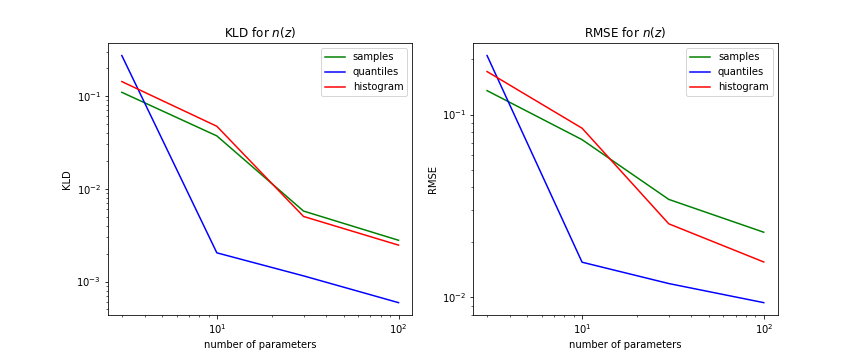
\includegraphics[width=0.9\columnwidth]{figures/stacked_placeholder.png}\\
  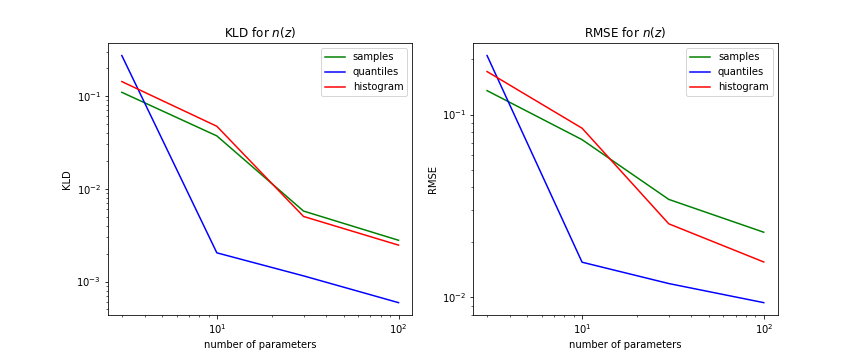
\includegraphics[width=0.9\columnwidth]{figures/stacked_placeholder.png}
  \caption{Placeholder! [$N_{f}$ (horizontal) vs. metric value (vertical), one 
color per format, curves from many instantiations of the subsample of galaxies 
(or error bars derived from those instantiations), one panel per dataset 
(vertical), panel title of dataset]
  \label{fig:stacked}}
\end{figure}

\COMMENT{Review relative performance and absolute differences of metric values. 
 Note $N_{f}$ at which asymptotic behavior is achieved for each format and rate 
of convergence to asymptote, across datasets.}

Further recommendations can be made if the requirements on the science products 
derived from the \pz\ catalog are known.  If the information loss tolerance on 
$n(z)$ for a given survey mission is specified, it would correspond to a 
horizontal line in Fig. \ref{fig:stacked}; the optimal format would be the one 
that drops below that line at the lowest value of $N_{f}$, which would be the 
optimal number of parameters to store.  We encourage the community to specify 
the requirements on estimators of science products like $n(z)$ in terms of 
information theoretic quantities such as entropy, as these are naturally 
relatable to \pz s.  We do not attempt to convert traditional percent 
error-based requirements to such a framework because it would require a fully 
probabilistic pipeline from \pz s to cosmological parameter constraints, which 
has not yet been developed.





\section{Conclusions \& Future Directions}
\label{sec:conclusions}


This work addresses how one may go about choosing a storage format and 
resolution for a catalog of \pz s for a survey of known data quality to balance 
the accuracy of the stored \pz s and the science metrics derived from them 
against the available storage resources.  We demonstrate the recommended method 
on two realistic mock datasets representative of upcoming \pz\ catalogs and 
draw the following conclusions:
\begin{itemize}
  \item \COMMENT{Insert observations of Sec. \ref{sec:results} here, 
emphasizing \pz\ data quality differences.}
  \item As indicated by the KLD, the quantile parametrization is a promising 
option for minimizing loss of information in \pz\ storage.
  \item Given the constraint that LSST will be able to store 200 floating point 
numbers to quantify the redshift of each galaxy and intends to include several 
\pz\ codes, we can safely say that LSST can store the output of more than one 
\pz\ code without any significant risk of loss of information.
\end{itemize}

We also make publicly available the \qp\ Python package central to this 
procedure and invite the community to contribute additional formats and metrics 
to the project.  \qp\ is a tool that can be used to optimize the choice of 
stored parametrization and number of stored parameters of a catalog of \pz s 
based on the accuracy needs of the use cases of the catalog.  Further 
applications of \qp\ functionality for manipulations of \pz s is demonstrated 
in the LSST-DESC PZ DC1 paper (in prep.).

We do not advocate for a one-size-fits-all solution to the problem and 
emphasize that the optimal choice must depend on the requirements of the 
science metric(s) and characteristics of the underlying \pz\ catalog.  
Furthermore, this procedure does not address the computational resources that 
may be necessary to perform the storage operation and to reconstruct \pz s into 
the format necessary for science calculations.

\dots


\subsection*{Acknowledgments}


This work was incubated at the 2016 LSST-DESC Hack Week.  We invite the 
following people to be co-authors: Melissa Graham, Sam Schmidt, [Buzzard team].

%
%This is the text imported from \code{acknowledgments.tex}, and will be replaced by some standard LSST DESC boilerplate at some point.
%


Author contributions are listed below. \\
A.I.~Malz: Initiated project, led development work. \\
P.J.~Marshall: Advised on statistics, and project design and management. \\
S.J.~Schmidt: Produced the PDFs for the fainter mock catalog. \\
M.L.~Graham: Produced the photometry and PDFs for the brighter mock catalog. \\
J.~DeRose: Produced the photometry for the fainter mock catalog. \\
R.~Wechsler: Supervised production of the fainter mock catalog. \\



\bibliography{lsstdesc,main}

\end{document}
